\chapter{Scopi e Problemi Affrontati}\label{capitolo1}
In questo capitolo verranno esposti gli scopi e i problemi incontrati durante l'attivit\`a di stage divisi in due argomenti.
In particolare si tratta lo sviluppo delle applicazioni per il MM \ref{cap:moduliproblemi} e lo sviluppo dell'interfaccia web
di amministrazione \ref{cap:interfacciaproblemi}

\section{Applicazioni del MagicMirror}\label{cap:moduliproblemi}
Il MagicMirror \`e un software che espone API, le quali permettono
l'integrazione di applicazioni sviluppate da terzi e forniscono funzionalit\`a per la comunicazione, gestione
ed organizzazione tra le applicazioni.
Lo scopo nello sviluppo delle applicazioni, durante lo stage, \`e stato
di creare programmi che permettessero l'interazione tra il software principale
e l'essere umano. Nello specifico si \`e voluto implementare la possibilit\`a, da parte di un utente,
di controllare le applicazioni attive sul MagicMirror tramite l'impartizione di comandi vocali
o movimenti delle dita su una scheda Touch Board.
In questa parte si \`e dovuto affrontare il problema di far comunicare
i diversi dispositivi hardware con il calcolatore principale, e di programmare
le applicazioni con linguaggi diversi, a seconda della compatibilit\`a di un linguaggio
e delle librerie a disposizione di una determinata periferica.
\\[2\baselineskip]

\section{Interfaccia di controllo del MagicMirror}\label{cap:interfacciaproblemi}
Il MM possiede all'interno delle sue cartelle un file di configurazione, il quale permette
di configurare sia MM che le applicazioni caricate su quest'ultimo.
Prima dello stage per modificare la configurazione, bisognava accedere direttamente al file di configurazione
appena presentato e modificarlo. Questo approccio, oltre ad essere scomodo, pu\`o anche
causare errori, dal momento che \`e necessaria una sintassi corretta all'interno del file.\\[1\baselineskip]
Preso atto di questo, nella seconda parte dello stage si \`e svolta la progettazione e lo sviluppo di un'interfaccia Web di configurazione remota
il cui scopo \`e di permettere ad un utente autenticato di gestire
le configurazioni del MM e dei moduli implementati su di esso da una pagina web,
senza dover accedere alla macchina fisica su cui gira l'applicazione ed implementando
una validazione per la sintassi del file di configurazione.
L'interfaccia permette anche di disattivare (o attivare) le applicazioni presenti nel MM,
la cui procedura, prima, richiedeva di aggiungere manualmente un pezzo di codice nella
configurazione del software principale.
Lo scambio dei messaggi tra il MM e la pagina web avviene in formato JSON, lo stesso formato
usato per il file di configurazione.\\
Un altro problema riscontrato in questa parte \`e stata la difficolt\`a dell'utilizzo di Javascript
perch\`e \`e un linguaggio orientato ad eventi, ovvero alcune funzioni vengono eseguite senza attendere
il risulato della precedente. Il linguaggio, per poter sincronizzare le funzioni, mette a disposizione
le callback: funzioni passate come parametro alla funzione principale che a loro volta avevano come paramentro il risultato,
in modo da poter eseguire le operazioni solo dopo che la funzione chiamante avesse prodotto l'output.
Senza buone pratiche di programmazione si rischia di incontrarsi in un fenomeno chiamato "Callback Hell", ovvero Callback che chiamano a loro volta
altre Callback creando funzioni annidate pi\`u volte, come mostrato in figura \ref{fig:hell}.
\begin{figure}[H]
    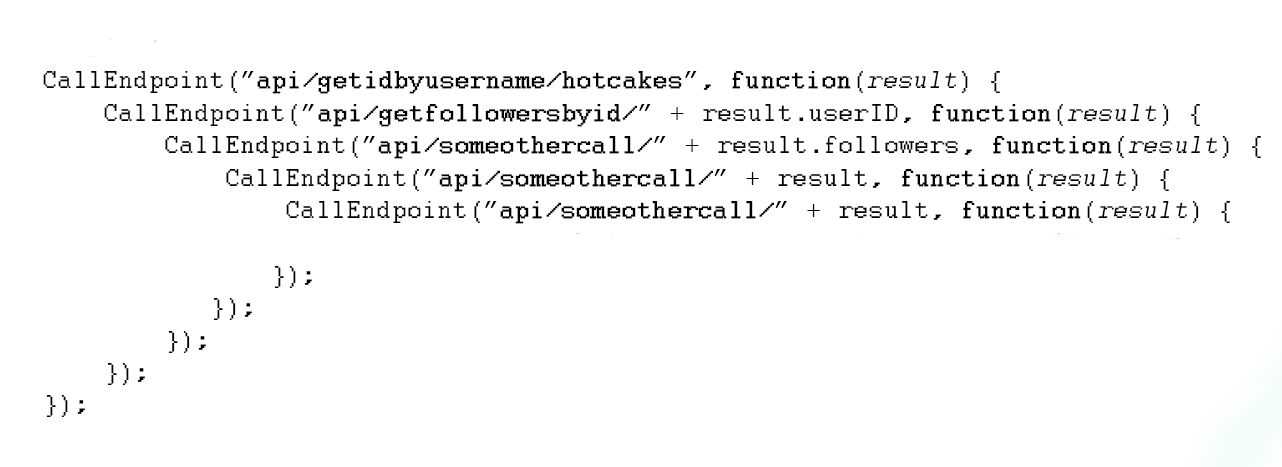
\includegraphics[width=1\textwidth, height=0.3\textheight]{callback}
    \caption{Esempio di Callback Hell}
    \label{fig:hell}
\end{figure}
Nella figura il codice esegue delle query attraverso delle API esposte da un servizio. La funzione \textit{CallEndpoint()} chiama la funzione dell'API passandogli
un percorso, il quale restituisce il risultato di una query. Per poter procedere a quella successiva \`e richiesto il risultato della precedente e
per farlo \`e necessario l'utilizzo di un'altra Callback. Questa dipendenza si ripresenta anche nelle query successive creando un annidamento
sempre maggiore conosciuto come CallbackHell.
